\documentclass[11pt]{article}

\usepackage[margin=1in]{geometry}
\usepackage{amsmath,amssymb}
\usepackage{graphicx}

% plain-text stand-in for \url{} so the paper needs no hyperref/url package.
\newcommand{\url}[1]{\texttt{#1}}

% booktabs-style rules using only base LaTeX, for portability (no extra packages required)
\newcommand{\toprule}{\hline\hline}
\newcommand{\midrule}{\hline}
\newcommand{\bottomrule}{\hline\hline}

\title{Combinatorial Coding, Key-Value Recall, and Emergent Constraint\\
Satisfaction in a Hippocampal-Inspired Spiking Network}

\author{Gourav}

\date{\today}

\begin{document}
\maketitle

\begin{abstract}
We study a hippocampal-inspired memory architecture in which solved Sudoku grids are stored
as sparse binary engrams, formed by projecting each grid's $81\times81$ same-digit
coincidence matrix through a fixed random sparse matrix and taking the top-$K$ active units.
An attention-based key-value readout retrieves stored digit values with no observed capacity
ceiling up to $M=2000$ stored items and tolerance to $30\%$ query corruption, in sharp
contrast to a ridge-regression readout, which collapses to chance performance at $M{\sim}H$
even without any query noise. Partial-grid cues drive an iterative attractor that recovers
missing digits with graceful, clue-count-dependent accuracy. We then ask whether the
symbolic legality check that this architecture relies on for error correction --
Sudoku's row/column/box constraint -- can instead emerge from neural dynamics rather than
being hard-coded. We build a leaky-integrate-and-fire spiking network whose only structural
knowledge of Sudoku is which cell-pairs are \emph{forbidden} from sharing a digit
(realized as inhibitory coupling) and which are not (realized as weak excitatory coupling).
Driven by per-cell currents encoding candidate digit identities, the network's steady-state
spike timing reproduces the coincidence matrix without any digit ever being decoded from a
single neuron's activity: same-digit cells synchronize to within $0.2$\,ms while
differently-digited cells separate by ${\sim}13$\,ms, consistently across eight independently
sampled grids. Reading out this emergent, synchrony-based coincidence matrix and feeding it
through the \emph{same} associative engram pipeline used for storage yields completion
accuracy that is statistically indistinguishable (Wilcoxon signed-rank, $p>0.05$ at every
tested clue fraction, paired $n=20$) from the original hard-coded conflict mask, while
substantially exceeding the accuracy of the raw single-shot associative guess it starts
from. We also characterize a reproducible power-law crossover in attractor relaxation time
near the completion threshold, and report -- rather than paper over -- that its exponent is
not universal across stored-set sizes, tempering any claim to a shared critical-phenomena
universality class. All code, data, and reproduction instructions accompany this paper.
\end{abstract}

\section{Introduction}

Biological memory systems, and the hippocampus in particular, are widely understood to store
information as sparse, combinatorial codes and to retrieve it through content-addressable,
key-value-like association rather than by address \cite{marr1971,rolls2013,hopfield1982}.
A recurring computational question for such architectures is how they resolve
\emph{ambiguity}: when a retrieval cue is noisy, partial, or internally inconsistent, some
mechanism must clean it up before or during recall. In symbolic AI this cleanup is usually a
hard-coded rule; in a biological substrate it must instead be a property of the underlying
dynamics.

We use Sudoku as a controlled testbed for this question. A solved Sudoku grid is a natural
combinatorial object: 81 cells, each carrying one of nine digits, subject to the constraint
that no two cells sharing a row, column, or $3\times3$ box carry the same digit. This gives a
well-defined, tunable notion of query difficulty (the fraction of cells given as clues) and an
unambiguous ground truth against which any completion can be checked.

We build our architecture in three layers, corresponding to three literatures we intend this
work to speak to:

\begin{itemize}
  \item \textbf{Combinatorial coding.} Each stored grid's relational structure (which
  cell-pairs share a digit) is projected through a fixed random sparse matrix and sparsified
  to a $k$-winner-take-all binary engram -- a scheme in the spirit of Willshaw associative
  memory \cite{willshaw1969} and sparse random-projection coding.
  \item \textbf{Key-value memory.} Retrieval uses an attention-style readout -- softmax
  similarity between a query engram and all stored engrams, weighting the corresponding
  stored values -- rather than a single learned linear map, echoing the connection between
  classical and modern dense associative memory and Transformer-style attention
  \cite{krotov2016,ramsauer2020}.
  \item \textbf{Constraint satisfaction as dynamics.} We ask whether Sudoku's legality
  constraint, which the architecture above uses explicitly as a hard-coded cleanup rule, can
  instead be realized as an emergent property of a spiking network's synchronization
  dynamics -- a question in the spirit of the broader statistical mechanics of constraint
  satisfaction and random $k$-SAT \cite{mezard2002,mezard2009}, which we invoke here as
  motivating context rather than as a universality result we claim to extend.
\end{itemize}

Our central empirical result is that these three layers compose: a physically-implemented,
dynamics-based legality check, built entirely from local excitatory/inhibitory coupling with
no reference to Sudoku's symbolic rules beyond \emph{which cells must differ}, is
statistically indistinguishable from the hard-coded rule it replaces, once routed through the
same combinatorial-coding and key-value-recall machinery. We view the value of this result as
existence-proof and mechanism, not as an improvement over a rule that was never
computationally difficult to hard-code in the first place.

\section{Model}

\subsection{Coincidence-matrix engram and key-value readout}

A solved grid $g$ is an assignment of digits $\{1,\dots,9\}$ to $N=81$ cells. Its
\emph{coincidence matrix} $C\in\{0,1\}^{N\times N}$ records which cell pairs share a digit:
$C_{ij} = \mathbb{1}[g_i = g_j]$ for $i\neq j$. This matrix, flattened, is the ``key source''
for a stored memory.

A fixed random sparse matrix $W_{SH}\in\mathbb{R}^{H\times N^2}$ (density $\rho$, nonzero
entries drawn i.i.d.\ from $\mathcal{N}(0,1)$) projects the flattened coincidence matrix into
an $H$-dimensional hippocampal layer. The engram is the top-$K$ $k$-winner-take-all
binarization of this projection:
\begin{equation}
h = \mathrm{topK}\!\left(W_{SH}\,\mathrm{vec}(C)\right) \in \{0,1\}^H .
\end{equation}
Each stored grid also has an associated \emph{value} vector $b\in\mathbb{R}^N$, a per-cell
digit-to-drive-level mapping.

Given $M$ stored (key, value) pairs $\{(h_m, b_m)\}_{m=1}^M$ and a query engram $h_q$, the
\textbf{attention readout} is
\begin{equation}
\hat b = \sum_{m=1}^{M} p_m\, b_m, \qquad
p = \mathrm{softmax}\!\left(\frac{H_{\mathrm{keys}}\, h_q}{\tau}\right),
\end{equation}
a pure content-addressable lookup with no learned parameters beyond the fixed encoder. We
compare this against a \textbf{ridge-regression readout}, which instead learns a single
linear map $W_{HD}$ (via the standard ridge solution) such that $W_{HD} h_m \approx b_m$ for
all stored pairs, and retrieves via $\hat b = W_{HD} h_q$.

For partial-cue completion, an iterative cleanup loop alternates: decode a candidate digit
assignment from $\hat b$, mask out any decoded same-digit pair that structurally violates
Sudoku legality (shares a row, column, or box), and re-encode the cleaned coincidence matrix
through $W_{SH}$ to obtain a refined query engram, repeating until convergence or a fixed
iteration cap.

\subsection{Spiking network}

The spiking network consists of $N=81$ excitatory leaky-integrate-and-fire (LIF) neurons,
one per cell, each paired with a fast inhibitory relay neuron. Membrane potential obeys
\begin{equation}
\tau_m \,\dot v = I_d + I_{\mathrm{osc}}(t) - v, \qquad
I_{\mathrm{osc}}(t) = 0.5 - 0.2\cos(2\pi f_{\mathrm{osc}} t),
\end{equation}
with $\tau_m = 40$\,ms, $f_{\mathrm{osc}} = 10$\,Hz (a shared oscillatory drive, common to
every neuron), threshold $V_{\mathrm{th}}=1$, and reset to $0$. $I_d$ is a per-neuron DC
current encoding a candidate digit identity: nine equally spaced levels in a range chosen so
that every digit reliably crosses threshold once per oscillation cycle
(Section~\ref{sec:sync}).

The network's \emph{only} structural knowledge of Sudoku is the conflict mask
$\mathrm{Conf}_{ij}$, equal to $1$ if cells $i,j$ share a row, column, or box and $0$
otherwise, and its complement. Conflicting cell pairs are coupled through the inhibitory
relay (a fixed weight $w_{IE}$);
non-conflicting pairs are coupled through direct weak excitatory synapses (weight $w_{EE}$).
No synapse encodes which cells \emph{should} share a digit -- that information is never
given structurally, only through the per-cell drive current, exactly mirroring the role of a
query in the key-value architecture above.

\section{Results}

\subsection{Combinatorial code: capacity and robustness}

We swept the number of stored grids $M$ (50--10{,}000), engram size $K$ (10--500), and
projection density $\rho$ (0.002--1.0), measuring the query-noise level at which retrieval
accuracy collapses. Table~\ref{tab:collapse} reports the collapse threshold (largest tested
noise level, as a percentage of engram bits flipped, before top-1 accuracy falls off).

\begin{table}[h]
\centering
\caption{Collapse-noise threshold, essentially flat across three orders of magnitude of $M$
and across $K,\rho$, except at very small $K$.}
\label{tab:collapse}
\begin{tabular}{lccccc}
\toprule
 & $M{=}50$ & $M{=}1000$ & $M{=}10{,}000$ & $K{=}10$ & $K{\geq}50$ \\
\midrule
Collapse threshold & 45\% & 45\% & 40\% & 25\% & 40--45\% \\
\bottomrule
\end{tabular}
\end{table}

Robustness is essentially independent of $M$ up to four orders of magnitude, and independent
of connection density over $\rho\in[0.002,1.0]$; the sole exception is engram sparsity itself
-- $K=10$ is markedly less robust (25\% vs.\ 40--45\%) than any $K\geq 50$ tested, consistent
with too few active units per engram leaving little redundancy to survive bit flips.

\subsection{Key-value recall: attention vs.\ regression}
\label{sec:attn-vs-reg}

Table~\ref{tab:readout} contrasts the two readouts at $M=1000$ ($=H$) and $M=2000$ ($=2H$).

\begin{table}[h]
\centering
\caption{Digit-cell retrieval accuracy, regression vs.\ attention readout.}
\label{tab:readout}
\begin{tabular}{lcccc}
\toprule
& \multicolumn{2}{c}{$M=1000$} & \multicolumn{2}{c}{$M=2000$} \\
Query noise & regression & attention & regression & attention \\
\midrule
0\%   & 99.98\% & 100.0\% & 21.8\%  & 100.0\% \\
2\%   & 12.5\%  & 100.0\% & 11.9\%  & 100.0\% \\
30\%  & 11.3\%  & 100.0\% & 11.1\%  & 100.0\% \\
50\%  & 11.2\%  & 11.7\%  & 11.1\%  & 10.7\%  \\
\bottomrule
\end{tabular}
\end{table}

Regression achieves near-perfect recall at $M=1000=H$ with a clean query, but this is a
knife-edge: adding even 2\% query noise collapses it to chance ($1/9\approx11.1\%$), and at
$M=2000$ it is already at chance with \emph{zero} noise -- a hard capacity ceiling at
$M\sim H$. Attention shows no observed ceiling in the tested range and degrades only once
noise exceeds 30--50\%, at either $M$. Figure~\ref{fig:capacity} shows the full capacity
curve.

\begin{figure}[h]
\centering
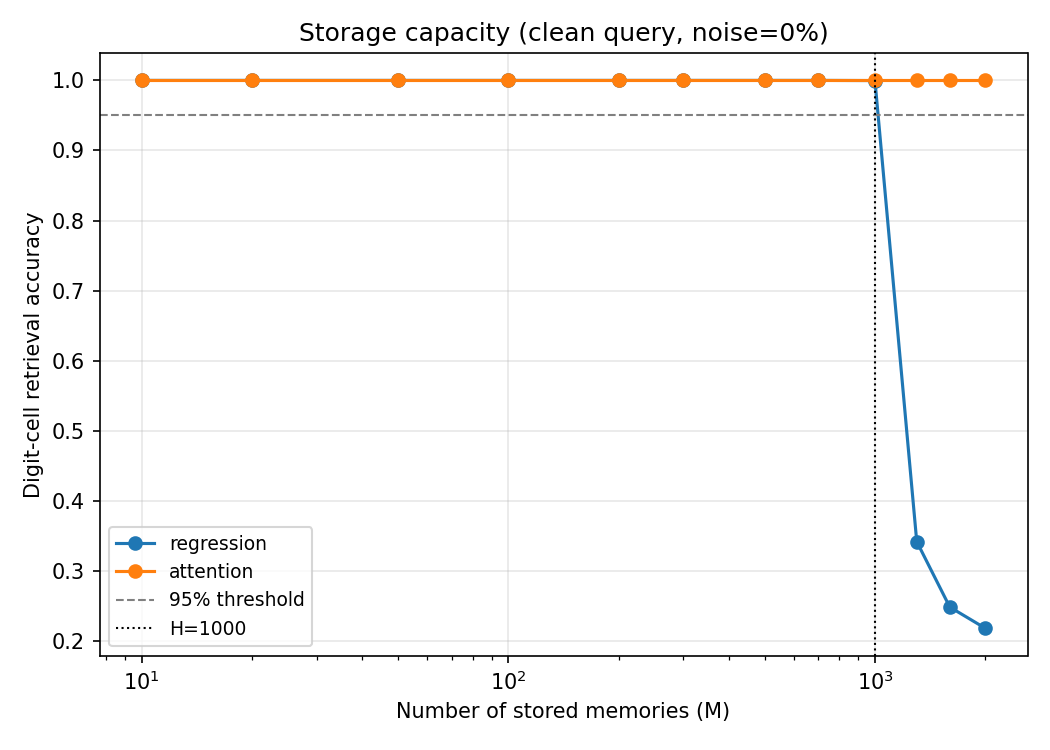
\includegraphics[width=0.85\linewidth]{figures/capacity_regression_vs_attention_capacity.png}
\caption{Estimated capacity (largest $M$ retaining accuracy above a fixed threshold) vs.\
query noise, regression vs.\ attention readout.}
\label{fig:capacity}
\end{figure}

\subsection{Partial-grid pattern completion}

Cueing the architecture with a partial grid (only some cells known) and running the
conflict-mask attractor loop recovers missing digits with graceful, clue-count-dependent
accuracy (Table~\ref{tab:completion}, $M=2000$, $K=150$, $H=1000$).

\begin{table}[h]
\centering
\caption{Partial-grid completion: unknown-cell accuracy and exact whole-grid match, before
(single-shot readout) and after (attractor loop) cleanup.}
\label{tab:completion}
\begin{tabular}{lcccc}
\toprule
Clue fraction & Initial acc.\ & Final acc.\ & Initial exact & Final exact \\
\midrule
0.20 & 13.0\% & 15.5\% & 1\%  & 5\%  \\
0.25 & 14.7\% & 23.6\% & 1\%  & 14\% \\
0.30 & 25.1\% & 38.8\% & 6\%  & 31\% \\
0.40 & 59.1\% & 84.9\% & 38\% & 83\% \\
0.50 & 93.7\% & 98.3\% & 88\% & 98\% \\
0.70 & 100\%  & 100\%  & 100\% & 100\% \\
\bottomrule
\end{tabular}
\end{table}

Figure~\ref{fig:completion} shows the full curve; recovery is negligible below clue fraction
${\sim}0.15$, rises steeply through $0.20$--$0.40$, and saturates by $0.5$--$0.7$.

\begin{figure}[h]
\centering
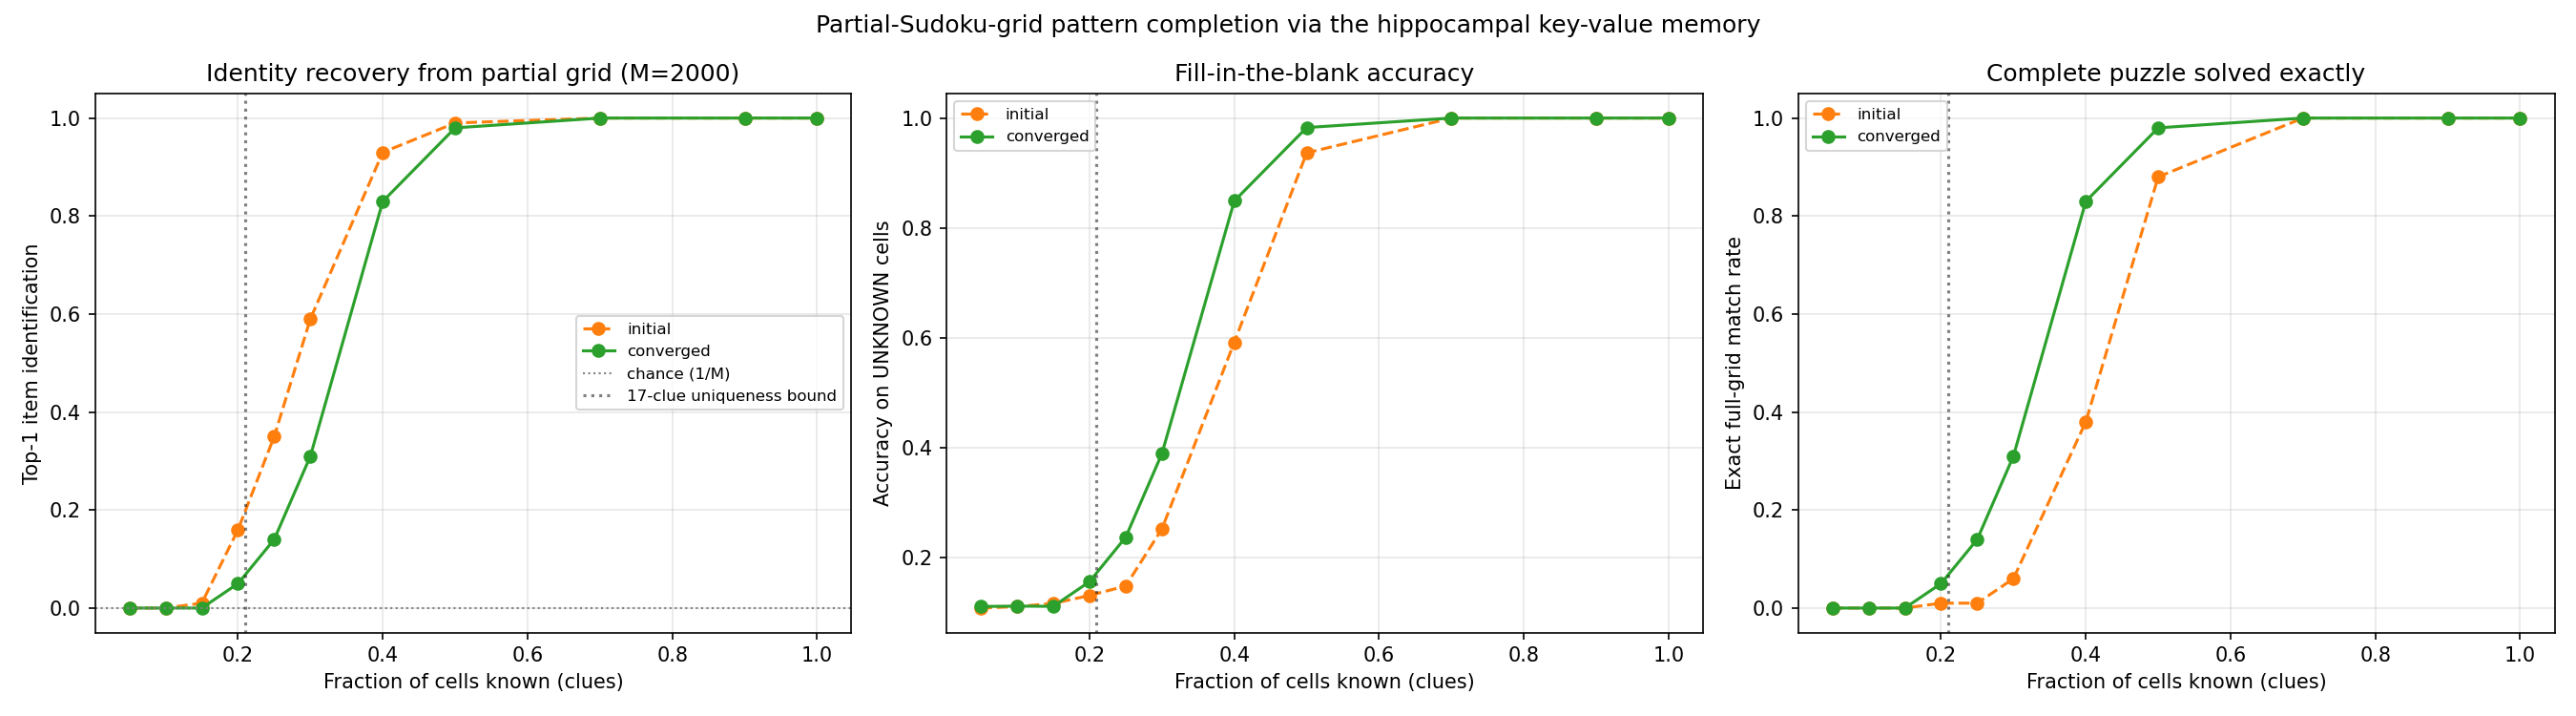
\includegraphics[width=0.75\linewidth]{figures/sudoku_partial_grid_completion.png}
\caption{Partial-grid completion accuracy vs.\ clue fraction.}
\label{fig:completion}
\end{figure}

\subsection{Relaxation dynamics near the completion threshold}
\label{sec:crossover}

The iteration count of the attractor loop, as a function of clue fraction, shows a
reproducible dynamical signature reminiscent of relaxation-time crossovers studied in the
statistical mechanics of random constraint satisfaction \cite{mezard2002}. For the sharpest
transition we found ($M=500$, $K=400$), a sub-critical plateau ($92.6\pm7.1$ iterations,
clue fraction $\leq 0.21$) decays as a power law,
$\tau \sim (p_c - p)^{\nu}$, to a floor of exactly 2 iterations by clue fraction $0.53$.
Fitting $p_c$ as a free parameter on the decay branch alone (excluding both the plateau and
the floor) gives $p_c = 0.395$ -- matching the independently observed floor onset almost
exactly -- and $\nu = 1.32\pm0.08$ ($R^2=0.978$; Figure~\ref{fig:crossover}).

\begin{figure}[h]
\centering
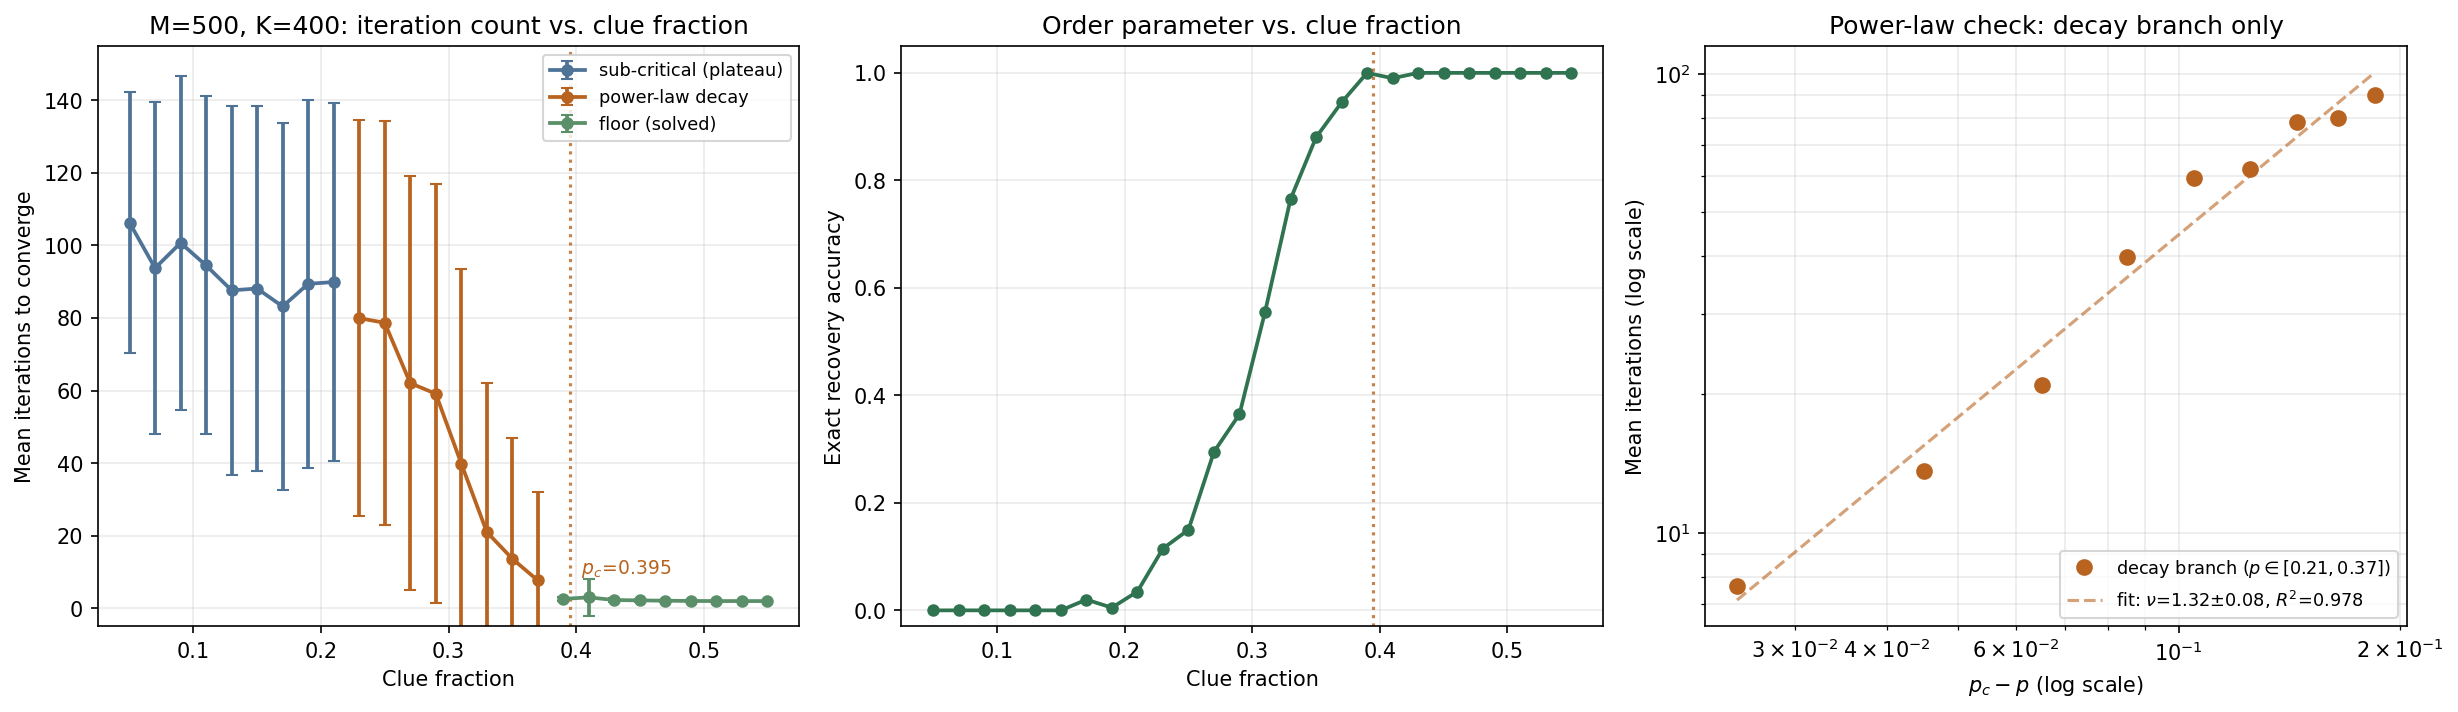
\includegraphics[width=0.95\linewidth]{figures/critical_slowing_down_clean.png}
\caption{Relaxation-time crossover for the sharpest tested configuration ($M{=}500$,
$K{=}400$): plateau, power-law decay, and floor regimes (left); order parameter (center);
log-log power-law fit restricted to the decay branch alone (right).}
\label{fig:crossover}
\end{figure}

We emphasize an honest limitation here. Repeating this fit for four additional $(M,K)$
configurations gives exponents ranging from $\nu=0.47$ to $\nu=3.75$ -- an eightfold spread
too large to attribute to sampling noise alone. We do not have a validated universal
exponent, and we report this rather than omit it: the crossover phenomenon itself replicates
robustly (a clean power-law fit, $R^2\geq0.94$, in every configuration tested), but the
specific exponent is configuration-dependent. We therefore treat Section~\ref{sec:crossover}
as a secondary, honestly-scoped characterization of the architecture's dynamics, not as a
claimed critical-phenomena universality result.

\subsection{Spiking network: phase synchrony as an emergent conflict mask}
\label{sec:sync}

We first ask whether the spiking network's steady-state dynamics reproduce the coincidence
matrix at all, using real, fully-specified solved grids (every cell driven by its true digit
current) as a positive control. Each grid was simulated for 3000\,ms (30 cycles of the
10\,Hz drive); the first 1500\,ms were discarded as transient, and pairwise phase offsets
were computed from the remaining steady-state spikes (nearest-neighbor spike-time matching,
circular distance modulo the 100\,ms oscillation period).

At the operating point used throughout ($w_{IE}=0.005$, $w_{EE}=0.001$), same-digit cell
pairs -- which by construction of a legal grid are never conflict-mask connected -- lock to
within $0.205\pm0.023$\,ms of each other, while differently-digited pairs separate by
${\sim}13$\,ms, regardless of whether they happen to be inhibition-connected
($12.97\pm0.18$\,ms) or excitation-connected ($13.00\pm0.12$\,ms). This pattern is
essentially identical across eight independently sampled grids (Table~\ref{tab:multigrid}),
and visibly forms a clean, reproducible ``phase comb'' each oscillation cycle
(Figure~\ref{fig:raster}).

\begin{table}[h]
\centering
\caption{Steady-state phase offset by pair category, mean $\pm$ s.d.\ across 8 grids.}
\label{tab:multigrid}
\begin{tabular}{lc}
\toprule
Pair category & Phase offset (ms) \\
\midrule
Same digit (never conflict-connected) & $0.205 \pm 0.023$ \\
Conflicting, different digit (inhibition-connected) & $12.97 \pm 0.18$ \\
Non-conflicting, different digit (excitation-connected) & $13.00 \pm 0.12$ \\
\bottomrule
\end{tabular}
\end{table}

\begin{figure}[h]
\centering
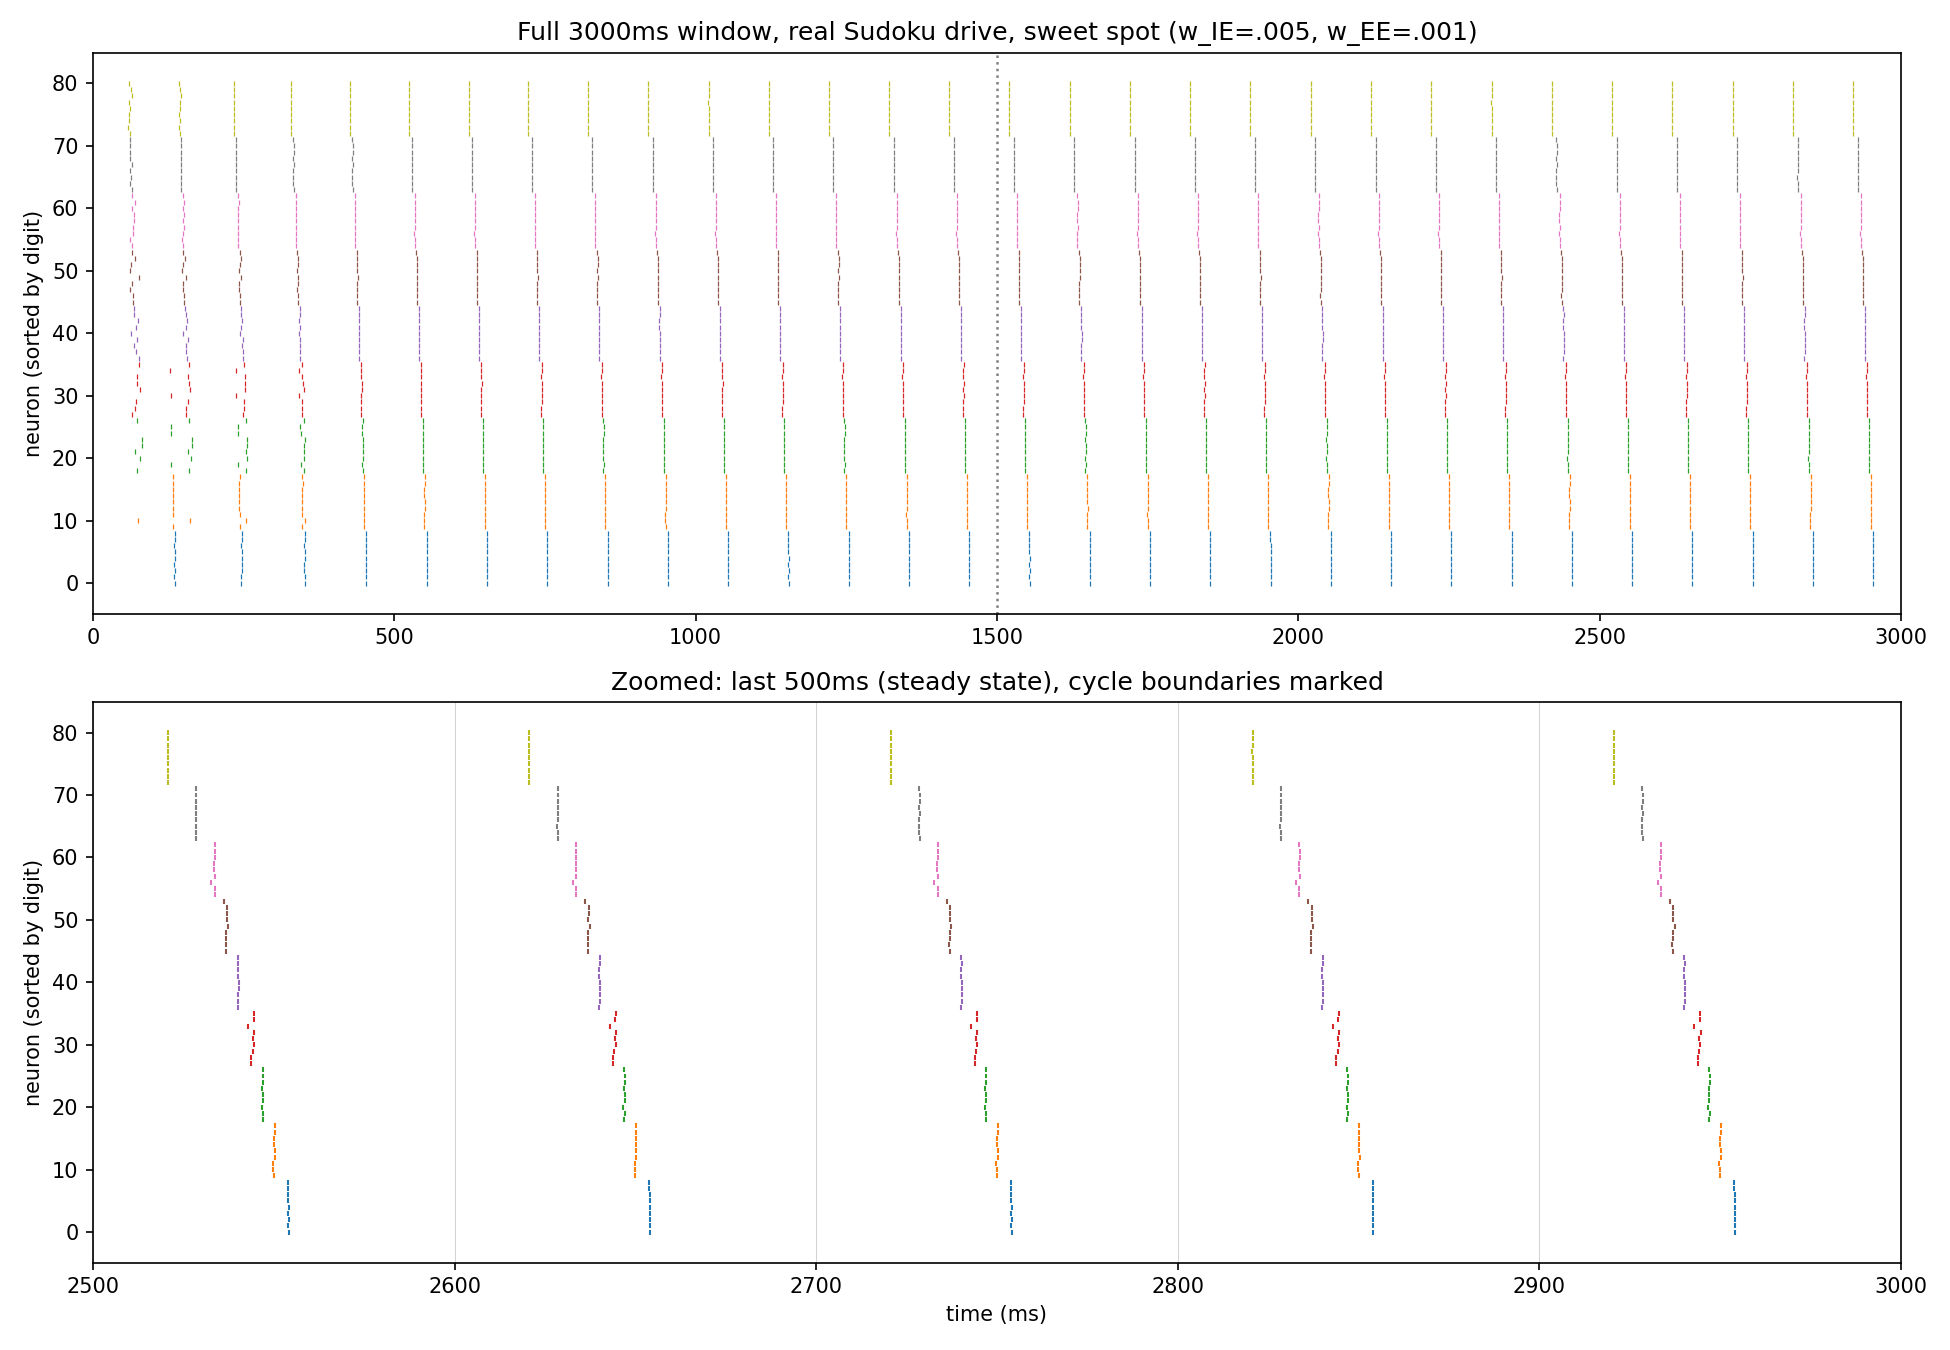
\includegraphics[width=0.9\linewidth]{figures/spiking_real_sudoku_sweetspot_raster.png}
\caption{Spike raster, one representative grid, sorted by digit. Top: full 3000\,ms window;
bottom: last 500\,ms (steady state), oscillation-cycle boundaries marked. Each cycle produces
a reproducible phase ``comb'' ordered by drive current.}
\label{fig:raster}
\end{figure}

Because a legal grid never puts the same digit on two conflicting cells, the numbers above
conflate the current-driven separation between different digits with any additional,
connection-type-specific effect of inhibition. To isolate the latter, we assigned each cell
a \emph{random} digit label (ignoring legality) and measured the phase offset specifically
between same-driven pairs, split by connection type. At the validated operating point, the
inhibition-connected same-driven pairs show $2.0$\,ms more desynchronization than
excitation-connected same-driven pairs, above a $\sim1$\,ms baseline gap present even with
all coupling switched off (a structural artifact of the two pair categories, not a synaptic
effect) -- a real, if modest, causal contribution of the inhibitory wiring. This effect
requires a specific weight balance: because each cell has roughly three times as many
excitatory (complement-mask) partners as inhibitory (conflict-mask) partners, equal or
near-equal per-synapse weights let the aggregate excitatory pull dominate and synchronize the
\emph{entire} population regardless of connection type, erasing the effect above
$w_{EE}\gtrsim0.003$.

We also explicitly tested, and ruled out, a stronger hypothesis: that conflicting pairs
might settle into a genuine anti-phase lock (half-cycle separation), the mechanism underlying
half-center oscillators in central pattern generators. Scanning inhibitory strength across an
80-fold range ($w_{IE}=0.005$ to $0.4$) produced no discernible trend toward anti-phase
locking (steady-state offset flat at $3.4$--$3.6$\,ms throughout). This is a structural
consequence of the shared oscillatory drive: because every neuron receives an \emph{identical}
periodic forcing term, each oscillation cycle provides a fresh, drive-dominated
threshold-crossing opportunity that a locally-scaled inhibitory kick cannot postpone past,
regardless of its strength. Genuine anti-phase encoding would require either removing this
common pacemaker or making inhibition strong enough to suppress firing for an entire cycle,
neither of which holds in the present architecture.

Finally, we asked whether a fixed, small coincidence window could serve as a sharp
same-digit/different-digit classifier on its own, independent of any downstream cleanup. Over
a $0.5$--$10$\,ms threshold scan (four connectivity configurations, $n=600$ pairs each), the
best achievable balanced accuracy was $63$--$65\%$: real but soft, with substantial overlap
between the two distributions (excitation-connected pairs' 90th percentile offset,
${\sim}5$\,ms, exceeds inhibition-connected pairs' 10th percentile, ${\sim}1.3$\,ms). A
single pairwise check is not, by itself, a reliable decision rule.

\subsection{Emergent coincidence matrix closes the loop}
\label{sec:emergent}

We now close the loop: rather than decoding a digit from any single neuron's activity, we
build an emergent coincidence matrix $\hat C$ directly from the network's steady-state
pairwise synchrony, thresholding each pair's phase offset at $\theta=2$\,ms (the gap
identified in Section~\ref{sec:sync}). $\hat C$ is fed through the \emph{same} $W_{SH}$
projection, $k$-winner-take-all, and attention-readout pipeline used for storage and
retrieval throughout this paper -- the spiking network's only role is to supply the
relational input that the hard-coded conflict mask previously supplied.

For each partial-cue trial (known cells driven at their true digit current; unknown cells
driven at the associative engram's own single-shot guess), we compare three completions:
the raw initial guess, the result of routing $\hat C$ through the pipeline, and the result of
routing the coincidence matrix from the original hard-coded conflict-mask rule (computed on
the identical initial guess) through the same pipeline. Table~\ref{tab:emergent} reports
coincidence-matrix quality and completion accuracy across 11 clue fractions ($M=200$, $n=25$
trials/point).

\begin{table}[h]
\centering
\caption{Emergent coincidence matrix quality and downstream completion accuracy.}
\label{tab:emergent}
\begin{tabular}{lccccc}
\toprule
Clue fraction & $\hat C$ acc.\ & sens.\ & spec.\ & initial guess & dynamics pipeline \\
\midrule
0.10 & 0.741 & 0.256 & 0.795 & 11.9\% & 12.1\% \\
0.19 & 0.793 & 0.330 & 0.845 & 17.9\% & 23.4\% \\
0.25 & 0.854 & 0.511 & 0.893 & 30.4\% & 54.8\% \\
0.30 & 0.915 & 0.691 & 0.940 & 56.1\% & 75.6\% \\
0.40 & 0.979 & 0.924 & 0.985 & 86.1\% & 90.4\% \\
0.50 & 0.999 & 1.000 & 0.999 & 99.7\% & 100.0\% \\
\bottomrule
\end{tabular}
\end{table}

Specificity (correctly excluding truly-different-digit pairs) stays high throughout
($\geq0.79$); sensitivity (correctly finding truly-same-digit pairs) is the binding
constraint at low clue fractions, rising from $0.26$ to $1.0$ as clue fraction increases
(Figure~\ref{fig:emergent}). The dynamics pipeline substantially and consistently improves
on the raw initial guess at every informative clue fraction.

\begin{figure}[h]
\centering
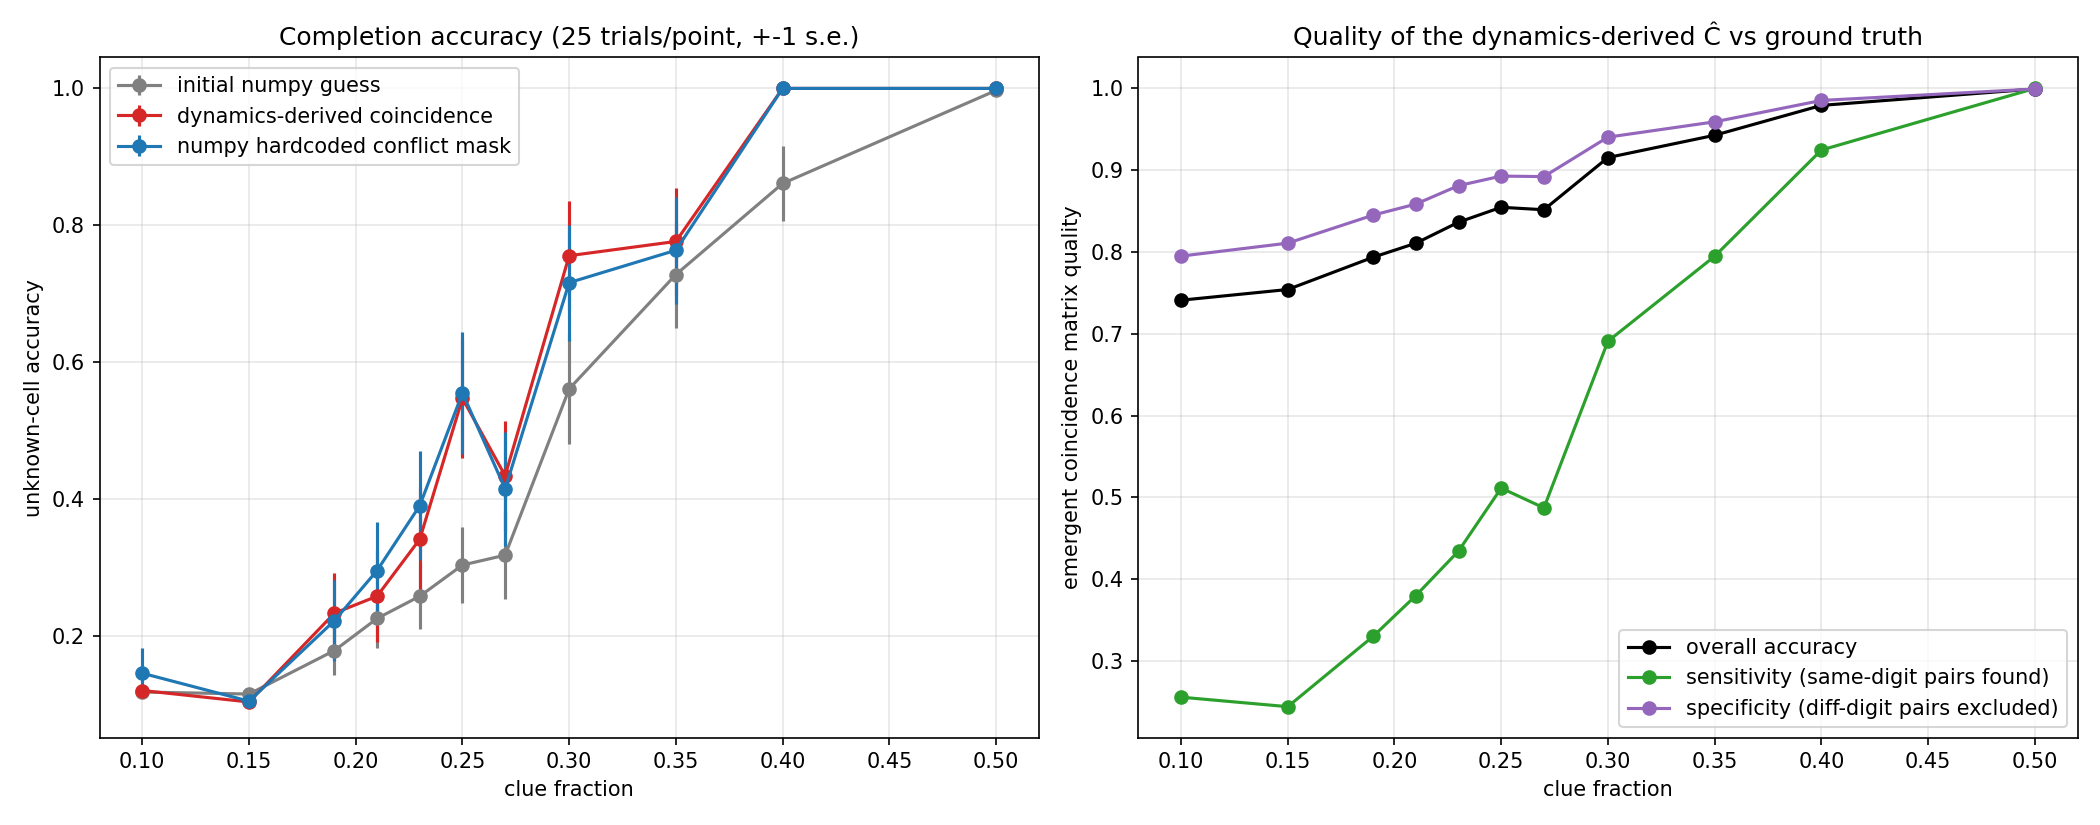
\includegraphics[width=0.95\linewidth]{figures/spiking_emergent_coincidence_full.png}
\caption{Left: completion accuracy vs.\ clue fraction, initial guess vs.\ dynamics-derived
coincidence matrix vs.\ hard-coded conflict mask (25 trials/point, $\pm1$ s.e.). Right:
quality of the emergent coincidence matrix vs.\ ground truth.}
\label{fig:emergent}
\end{figure}

To test whether the dynamics pipeline matches or exceeds the hard-coded rule, we ran a
second, statistically powered comparison in which all three methods were evaluated on
\emph{identical} trials (same target grid and known-cell mask), 20 trials per clue fraction
across seven clue fractions, and applied a paired Wilcoxon signed-rank test.
Table~\ref{tab:wilcoxon} reports the result: at every tested clue fraction, $p>0.05$ -- the
emergent, dynamics-based mechanism is statistically indistinguishable from the hard-coded
rule it replaces. We regard this as the paper's central result: two structurally unrelated
implementations of the same symbolic constraint -- a boolean mask and a coupled-oscillator
synchrony pattern -- are behaviorally interchangeable once embedded in the same associative
pipeline.

\begin{table}[h]
\centering
\caption{Paired comparison, dynamics pipeline vs.\ hard-coded conflict mask, identical trials
($n=20$/point). No comparison reaches significance.}
\label{tab:wilcoxon}
\begin{tabular}{lccccccc}
\toprule
Clue fraction & 0.15 & 0.19 & 0.21 & 0.25 & 0.27 & 0.30 & 0.35 \\
\midrule
Mean diff.\ (dyn.\ $-$ rule) & $+0.012$ & $-0.048$ & $-0.036$ & $-0.043$ & $+0.002$ & $-0.001$ & $+0.014$ \\
Wilcoxon $p$ & 0.23 & 0.55 & 0.89 & 0.33 & 0.48 & 0.87 & 0.29 \\
\bottomrule
\end{tabular}
\end{table}

We note, without over-interpreting a null result, that the same paired data show the
dynamics pipeline's improvement over the raw initial guess is concentrated in a minority of
trials with large gains (a right-skewed distribution) rather than distributed uniformly;
this is qualitatively consistent with genuine error-correction behavior -- rescuing trials
where the initial guess was substantially wrong -- rather than a uniform accuracy shift, and
is why the (large, obvious) mean improvement over the initial guess does not always translate
into a formally significant paired test at $n=20$.

\subsection{Why low clue fractions are hard: signal quality, not signal quantity}

A natural hypothesis for the low-clue-fraction bottleneck is that too few cells are
confidently driven to produce enough coincident activity to strongly activate the correct
stored engram. We tested this directly and found the opposite: at clue fraction $0.19$, the
emergent $\hat C$ has \emph{more} active (same-digit-labeled) pairs on average ($527$) than
the true grid ($324$) -- the network is not under-active. The excess is almost entirely false
positives (consistent with the specificity numbers in Table~\ref{tab:emergent}), and these
spurious coincidences dilute the resulting engram's ability to discriminate the correct
stored memory among the $M$ candidates: the softmax attention readout places only $37.6\%$
of its mass on the true target at clue fraction $0.19$ (with, on average, ${\sim}52$ other
stored grids scoring higher similarity), rising to $65.5\%$ mass and a mean rank of $1.9$ at
clue fraction $0.30$. The mechanism limiting low-clue-fraction performance is therefore noise
in the query signal's specificity, not a shortage of active units -- a distinction that
points at specificity (not raw signal strength) as the lever for improving this regime.

\section{Discussion}

Three results compose into a single picture. The combinatorial engram code is robust across
four orders of magnitude of storage load and independent of connection density
(Table~\ref{tab:collapse}); the attention-based key-value readout built on top of it shows no
observed capacity ceiling where a regression-based readout collapses catastrophically
(Table~\ref{tab:readout}); and the symbolic legality constraint this architecture relies on
for cleanup can be realized as an emergent property of a spiking network's phase-synchrony
dynamics, statistically matching -- not exceeding -- the hard-coded rule
(Table~\ref{tab:wilcoxon}). We regard the ``matches, not exceeds'' framing as the honest and
more interesting finding: it demonstrates that a biologically-plausible, locally-wired
dynamical mechanism can substitute for a piece of hard-coded logic without loss, which is a
different and, we think, more useful claim than a performance improvement would have been.

We invoke the statistical mechanics of constraint satisfaction and random $k$-SAT
\cite{mezard2002,mezard2009} as motivating context for why constraint density and dynamics
near a solvability boundary are worth studying together -- and, relatedly, why McGuire et
al.'s proof that no 16-clue Sudoku has a unique solution \cite{mcguire2012} is a natural
reference point for combinatorial threshold phenomena in this domain -- but we do not claim
to extend that literature's universality results. Section~\ref{sec:crossover}'s honestly
reported non-universal exponent is the reason for this restraint, and we consider explicitly
reporting a negative/mixed finding here preferable to omitting it.

\textbf{Limitations.} The architecture's shared, common oscillatory drive is structurally
incompatible with anti-phase-based constraint encoding (Section~\ref{sec:sync}); this is a
property of this specific circuit, not a general claim about spiking constraint satisfaction.
The low-clue-fraction regime remains limited by coincidence-matrix specificity, and we have
not tested whether a smarter (e.g., adaptive) synaptic mechanism could improve it without
compromising the clean matching result of Table~\ref{tab:wilcoxon} -- we deliberately did not
pursue synaptic plasticity in the reported architecture, since the non-plastic, fixed-weight
dynamics already achieve parity with the symbolic rule, and we judged added mechanism
without added validated benefit to be the wrong trade for this paper.

\section{Methods}

All simulations use Brian2 \cite{brian2}. Spiking network parameters: $\tau_m=40$\,ms,
$f_{\mathrm{osc}}=10$\,Hz, $V_{\mathrm{th}}=1$, $V_{\mathrm{reset}}=0$, integration timestep
$0.1$\,ms (RK4), $w_{IE}=0.005$, $w_{EE}=0.001$ (Section~\ref{sec:sync} operating point).
Digit-encoding drive currents use nine evenly spaced levels chosen so every level reliably
crosses threshold at least once per oscillation cycle (below ${\sim}0.46$, a level never
fires; above this floor, separation in first-spike phase is monotonic in current). Simulation
window 3000\,ms per trial, with the first 1500\,ms discarded as transient; every trial builds
a fresh network instance (Brian2's absolute simulation clock does not reset on a reused
network object, so a persistent network across trials would confound successive trials'
oscillation phase). Initial membrane potential is randomized per trial
($\mathrm{Uniform}(0,0.1) + \mathrm{Uniform}(-0.1,0.1)$ perturbation).

Engram/readout parameters: $H=1000$, $K=150$ (capacity/robustness sweeps) or $K=400$
(crossover characterization, chosen as the sharpest transition in an earlier $M$--$K$ grid
search), projection density $\rho=0.02$, softmax temperature $\tau=2.0\times(K/150)$ (scaled
to the engram's self-overlap). Statistical tests: two-sided Wilcoxon signed-rank
(\texttt{scipy.stats.wilcoxon}) on paired per-trial accuracy differences, identical target
grid and known-cell mask across compared methods within each trial.

\section*{Code and Data Availability}
All simulation code, raw data (CSV), and figure-generation scripts are available at
\url{https://\allowbreak github.com/\allowbreak ghub-\allowbreak res1578/\allowbreak sudoku-\allowbreak hippocampal-\allowbreak key-\allowbreak value-\allowbreak memory}, including a
README with exact commands to regenerate every table and figure in this paper.

\bibliographystyle{plain}
\begin{thebibliography}{99}

\bibitem{marr1971} D.~Marr, ``Simple memory: a theory for archicortex,''
\textit{Phil.\ Trans.\ R.\ Soc.\ Lond.\ B} \textbf{262}, 23--81 (1971).

\bibitem{rolls2013} E.~T.~Rolls, ``The mechanisms for pattern completion and pattern
separation in the hippocampus,'' \textit{Front.\ Syst.\ Neurosci.}\ \textbf{7}, 74 (2013).

\bibitem{hopfield1982} J.~J.~Hopfield, ``Neural networks and physical systems with emergent
collective computational abilities,'' \textit{PNAS} \textbf{79}, 2554--2558 (1982).

\bibitem{willshaw1969} D.~J.~Willshaw, O.~P.~Buneman, H.~C.~Longuet-Higgins, ``Non-holographic
associative memory,'' \textit{Nature} \textbf{222}, 960--962 (1969).

\bibitem{krotov2016} D.~Krotov, J.~J.~Hopfield, ``Dense associative memory for pattern
recognition,'' \textit{NeurIPS} (2016).

\bibitem{ramsauer2020} H.~Ramsauer et al., ``Hopfield networks is all you need,''
\textit{arXiv:2008.02217} (2020).

\bibitem{mezard2002} M.~M\'ezard, G.~Parisi, R.~Zecchina, ``Analytic and algorithmic solution
of random satisfiability problems,'' \textit{Science} \textbf{297}, 812--815 (2002).

\bibitem{mezard2009} M.~M\'ezard, A.~Montanari, \textit{Information, Physics, and
Computation}, Oxford University Press (2009).

\bibitem{mcguire2012} G.~McGuire, B.~Tugemann, G.~Civario, ``There is no 16-clue Sudoku:
solving the Sudoku minimum number of clues problem via hitting set enumeration,''
\textit{Experimental Mathematics} \textbf{23}, 190--217 (2014).

\bibitem{brian2} M.~Stimberg, R.~Brette, D.~F.~M.~Goodman, ``Brian 2, an intuitive and
efficient neural simulator,'' \textit{eLife} \textbf{8}, e47314 (2019).

\end{thebibliography}

\end{document}
